% ****** Start of file apssamp.tex ******
%
%   This file is part of the APS files in the REVTeX 4.2 distribution.
%   Version 4.2a of REVTeX, December 2014
%
%   Copyright (c) 2014 The American Physical Society.
%
%   See the REVTeX 4 README file for restrictions and more information.
%
% TeX'ing this file requires that you have AMS-LaTeX 2.0 installed
% as well as the rest of the prerequisites for REVTeX 4.2
%
% See the REVTeX 4 README file
% It also requires running BibTeX. The commands are as follows:
%
%  1)  latex apssamp.tex
%  2)  bibtex apssamp
%  3)  latex apssamp.tex
%  4)  latex apssamp.tex
%
\documentclass[%
 reprint,
%superscriptaddress,
%groupedaddress,
%unsortedaddress,
%runinaddress,
%frontmatterverbose, 
%preprint,
%preprintnumbers,
%nofootinbib,
%nobibnotes,
%bibnotes,
 amsmath,amssymb,
 aps,
%pra,
%prb,
%rmp,
%prstab,
%prstper,
%floatfix,
]{revtex4-2}
\usepackage{kotex}
\usepackage{physics}
\usepackage{graphicx}% Include figure files
\usepackage{dcolumn}% Align table columns on decimal point
\usepackage{bm}% bold math
%\usepackage{hyperref}% add hypertext capabilities
%\usepackage[mathlines]{lineno}% Enable numbering of text and display math
%\linenumbers\relax % Commence numbering lines

%\usepackage[showframe,%Uncomment any one of the following lines to test 
%%scale=0.7, marginratio={1:1, 2:3}, ignoreall,% default settings
%%text={7in,10in},centering,
%%margin=1.5in,
%%total={6.5in,8.75in}, top=1.2in, left=0.9in, includefoot,
%%height=10in,a5paper,hmargin={3cm,0.8in},
%]{geometry}

\def\rcurs{{\mbox{$\resizebox{.16in}{.08in}{
\includegraphics{ScriptR}}$}}}
\def\brcurs{{\mbox{$\resizebox{.16in}{.08in}{
\includegraphics{BoldR}}$}}}
\def\hrcurs{{\mbox{$\hat \brcurs$}}}

\begin{document}


\title{프랑크-헤르츠 실험 보고서}

\author{서울대학교 전기정보공학부 2018-12432 박정현}
 \email{alexist@snu.ac.kr}
\date{실험일자 : 11.13.2023}% It is always \today, today,
             %  but any date may be explicitly specified

\begin{abstract}
본 실험에서는 디락방정식을 이
\end{abstract}

%\keywords{Suggested keywords}%Use showkeys class option if keyword
                              %display desired
\maketitle

%\tableofcontents

\section{Introudction}
에너지의 양자화는 현대물리의 가장 중요한 원리이다. 특히 원자의 에너지가 양자화되어 있음을 보인 것은 매우 중요한 일이다. 독일의 물리학자 프랑크와 헤르츠는 1914년 원자 기체에 전기장을 가하여 전류값을 측정하여 내부 에너지가 양자화 되어 있음을 보였다. 본 실험에서는 플랑크, 헤르츠가 수행했던 실험을 재현하고 이를 통해 원자 내부의 에너지가 양자화 되어 있음을 간접적으로 증명하고 열전자, 원자의 에너지에 대한 이해도를 높인다.

\subsection{Ne 에너지 레벨}
Ne의 에너지 레벨은 Fig.\ref{fig:Neenergy}와 같다.[1] 19eV이상의 에너지를 가진 전자와 충돌하게 되면 3s, 3p와 같은 state로 1s,2s, 혹은 2p level의 전자가 excite하게 된다. 3s$\rightarrow$3p, 3s$\rightarrow$2p, 2s$\rightarrow$2p 혹은 2p$\rightarrow$1s으로의 전이가 발생하게 된다.

\begin{figure}[htbp]
	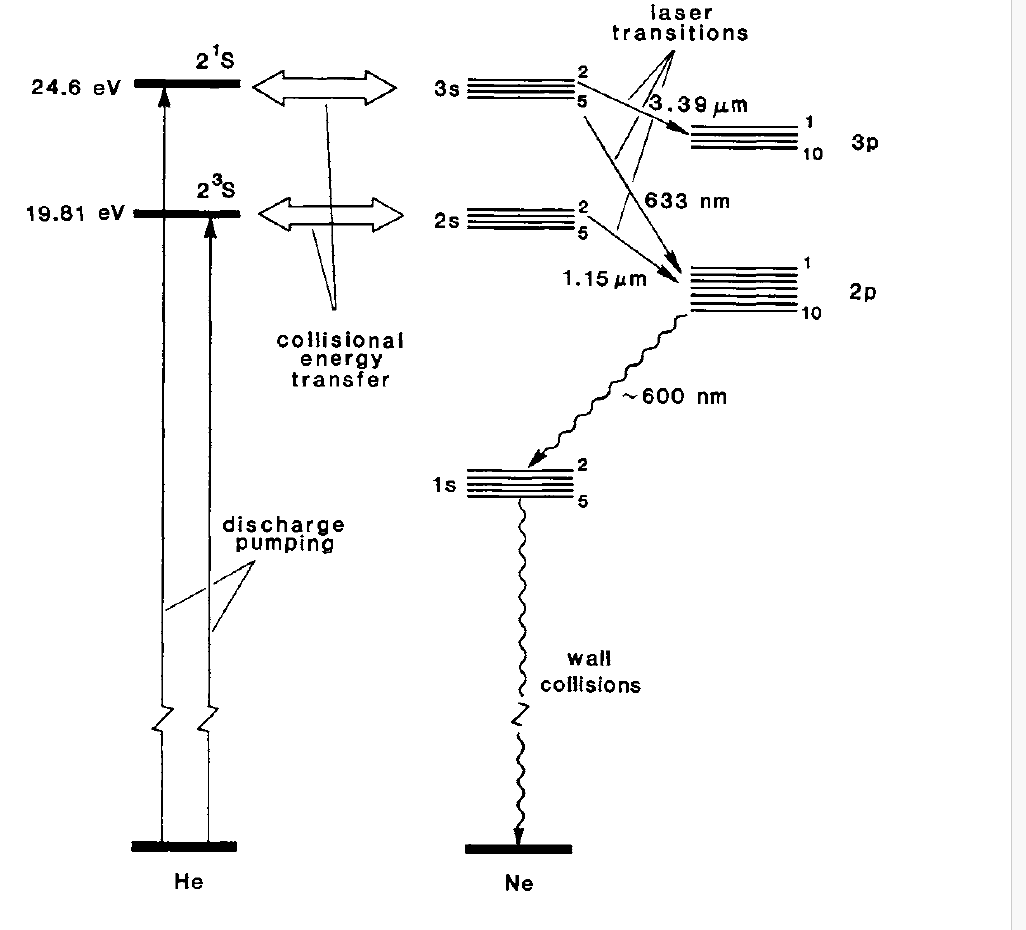
\includegraphics[width = 0.85\linewidth]{Neenergy.png}% Here is how to import EPS art
	\caption{\label{fig:Neenergy}Ne 원자 에너지 레벨}
\end{figure}

원자의 전자를 용수철 상수로 근사하여도 어느정도의 광학적 성질을 분석하는데 큰 문제가 발생하지 않는다. $\omega$의 주파수를 가진 전기장 내에서 이때 전자의 운동은 아래와 같이 풀어 낼 수 있다.
\begin{align}
	m(\ddot{\vec{x}}+\Gamma_{0}\dot{\vec{x}} + \omega_{0}^{2}\vec{x}) &= e\vec{E}_{0}\exp(-i\omega t)
\end{align}
가속하는 전자가 방출하는 power는 아래와 같은 방법을 통해 계산할 수 있다.
\begin{align}
	P &= \frac{e^{2}}{6\pi\varepsilon_{0}c^{3}}\frac{1}{2}\Re[\ddot{x}\ddot{x}^{*}]\\
	&= \frac{e^{4}\omega^{4}}{6\pi\varepsilon_{0}^{2}c^{4}m^{2}} \frac{I_{0}}{(\omega_{0}^{2}-\omega^{2})^{2}+\Gamma_{0}^{2}\omega^{2}}
\end{align}
$I_{0}$는 입사하는 전자기파의 에너지이다. 따라서 전자의 scattering cross section은 아래와 같다.
\begin{align}
	\sigma_{sc} &= \frac{e^{4}\omega^{4}}{6\pi\varepsilon_{0}^{2}c^{4}m^{2}} \frac{1}{(\omega_{0}^{2}-\omega^{2})^{2}+\Gamma_{0}^{2}\omega^{2}}
\end{align}
앞서 계산한 식은 전자기파에 대해서 풀은 식이지만 고전적인 영역에서 광자가 아닌 전자를 통해 에너지가 전달된다는 analogy를 이용하면 앞서 계산한 cross section을 사용해도 무방할 것이다. 즉, $eV = \hbar \omega$로 두어 전자의 에너지를 $\omega$로 대응시켜 식을 사용할 수 있다. 열전자들이 가속되어 Ne gas주변에 시간에 따라 일정한 수의 전자가 존재하는 경우 전류는 아래와 같은 Child-Langmuir법칙에 따라 흐르게 된다. [2]

\begin{align}
	J &= KV^{3/2}/d^{2}
\end{align}

하지만 전자와 Ne 원자가 충돌하는 경우 전자의 운동 에너지는 Ne원자의 전자로 전달되고 전자는 더 작아진 운동에너지를 가지고 scattering하게 된다.  따라서 Ne가스와 충돌하는 기체들이 존재하는 경우 해당 전자들은 에너지를 잃은 속도로 anode에 도달하게 되므로 전류량은 감소하게 될 것이다. Ne 원자의 총 갯수가 N, 그리고 단면적 A의 관에 존재하는 경우 전체 전자들중 충돌하는 비율을 $\eta$라고 했을 때 $\eta$는 아래의 식을 만족한다.

\begin{align}
	\eta &= \frac{N\sigma_{sc}}{A}
\end{align}

전자가 Ne원자를 excite시킬 만큼 충분한 에너지를 가지게 되는 위치를 $d_{0}$라고 할 때 $d_{0}$부터 다시 가속하게 되고 이러한 전자가 $d_{0}$에서 $d$까지 random하게 위치한다고 가정하면 감소하는 전류량은 아래의 식을 만족하면서 감소하게 된다. 단, $\omega \simeq \omega_{0}$ 주변에서의 적분값만 충분히 큰 값을 가지므로 $\eta$ 를 적분 밖으로 꺼내고 $d_{0}\simeq d$로 근사한다.

\begin{align}
	\Delta J &= -\frac{1}{d-d_{0}}\int_{d_{0}}^{d} \eta KV^{3/2}(1-\frac{x}{d})^{3/2}/(d-x)^{2}dx\\
	&\simeq -\frac{N}{A}\frac{e^{4}\omega^{4}}{6\pi\varepsilon_{0}^{2}c^{4}m^{2}}\frac{ KV^{3/2}}{(\omega_{0}^{2}-\omega^{2})^{2}+\Gamma_{0}^{2}\omega^{2}}\frac{1}{d^{2}}
\end{align}


따라서 총 전류는 아래와 같이 나타난다.

\begin{align}
	\begin{aligned}
	J_{tot} &\simeq KV^{3/2}/d^{2}\left(1-\frac{\beta}{(V-V_{0})+\gamma^{2}} \right)
	\end{aligned}
\end{align}

전자가 여러번 충돌하는 경우 아래의 식을 만족한다. $\beta_{1} = 0.01$, $\beta_{2} = 0.02$, $\beta_{3} = 0.03$, $\gamma_{1} = 0.01$, $\gamma_{2} = 0.02$, $\gamma_{3} = 0.03$, K=1, d=1 을 대입하여 계산한 이론적인 전류값은 Fig.\ref{fig:SIM}와 같다.

\begin{align}
	\begin{aligned}
	J_{tot} &= KV^{3/2}/d^{2}\Bigg(1-\frac{\beta_{1}}{(V-V_{0})+\gamma_{1}^{2}} \\
	&-\frac{\beta_{2}}{(V-2V_{0})+\gamma_{2}^{2}} -\frac{\beta_{3}}{(V-3V_{0})+\gamma_{3}^{2}} \cdots \Bigg)
	\end{aligned}
\end{align}

\begin{figure}[htbp]
	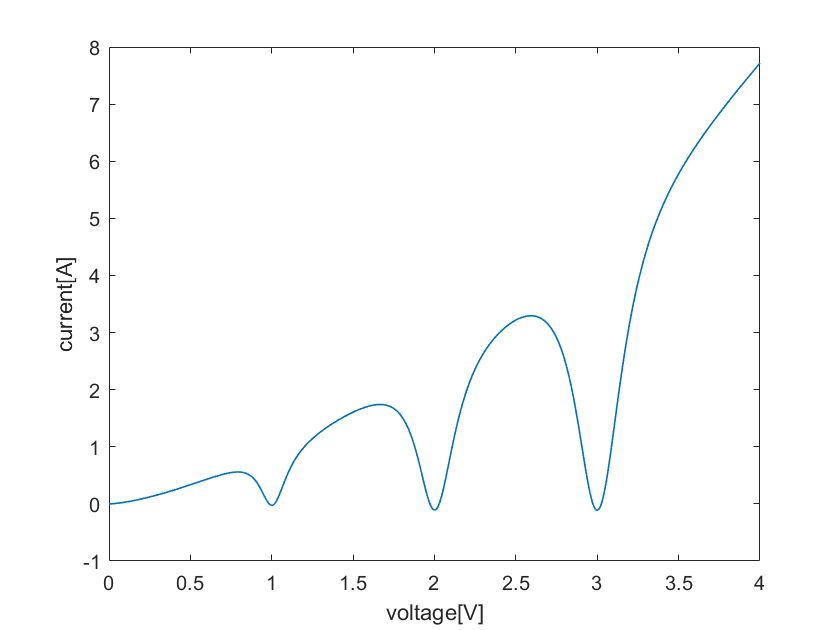
\includegraphics[width = 0.85\linewidth]{SIM.png}% Here is how to import EPS art
	\caption{\label{fig:SIM}Voltage vs Current 이론적 예측}
\end{figure}


\section{\label{sec:level1}Reference}
[1] Anthony E. Siegman - Lasers, An Introduction to Lasers, p. 65

[2] 그리피스 차일드 랭뮤어 법칙














[x] Griffiths, D. J. (2017, January 1). Quantum Mechanics in Three Dimensions. In \textit{Introduction to Quantum Mechanics}. (pp. 131-154). Cambridge University Press.

[2] Foot, C. (2005, January 1). Fine structure in the LS-coupling scheme. In \textit{Atomic Physics} (pp. 90–92). Oxford University Press.

[3] Griffiths, D. J. (2014, January 13). Relativistic Electrodynamics. In \textit{Introduction to Electrodynamics}. Pearson Higher Ed. ( p. 559)

[4] Foot, C. (2005, January 1). The interaction of atoms with radiation. In \textit{Atomic Physics} (p. 134). Oxford University Press.

[5] 제원호, Atomic Physics, 2nd Semester, 2019

[6] Foot, C. (2005, January 1). Fine structure in the LS-coupling scheme. In \textit{Atomic Physics} (p. 92). Oxford University Press.

[7] Foot, C. (2005, January 1). The hydrogen atom. In \textit{Atomic Physics} (pp. 40–41). Oxford University Press.

[8]  Foot, C. (2005, January 1). The hydrogen atom. In \textit{Atomic Physics} (pp. 30–31). Oxford University Press.

[10] M-Labs. (n.d.). M-Labs. https://m-labs.hk/experiment-control/artiq/

[11] Clark, S. M., Lobser, D., Revelle, M. C., Yale, C. G., Bossert, D., Burch, A. D., Chow, M. N., Hogle, C. W., Ivory, M., Pehr, J., Salzbrenner, B., Stick, D., Sweatt, W., Wilson, J. M., Winrow, E., \& Maunz, P. (2021). Engineering the Quantum Scientific Computing Open User Testbed. \textit{IEEE Transactions on Quantum Engineerin}g, 2, 1–32. https://doi.org/10.1109/tqe.2021.3096480

[12]  Foot, C. (2005, January 1). The interaction of atoms with radiation. In \textit{Atomic Physics} (p. 139). Oxford University Press.
\end{document}
%
% ****** End of file apssamp.tex ******
